\item \textbf{{[}HCI/PRELIM/9597/2016/P1/Q3{]} }

A transport company has a number of vehicles which can carry passengers.
Each vehicle is classified either as a bus or as a coach. All vehicles
have a registration number and have a certain number of seats for
the passengers. A bus can have a maximum number of standing passengers,
but a coach is not allowed to carry any standing passengers. Some
of the coaches are fitted with seat belts, but seat belts are never
fitted in a bus.

The transport company currently has a data file,\texttt{ VEHICLE.dat},
stores the following data:
\begin{itemize}
\item \texttt{RegNo} is used to uniquely identify a particular vehicle.
A typical vehicle registration number comes in the format \textquotedbl SBA1234\textquotedbl :
\begin{itemize}
\item S -- vehicle class (\textquotedbl S\textquotedbl{} stands for a
private vehicle) 
\item BA -- alphabetical series (\textquotedbl I\textquotedbl{} and \textquotedbl O\textquotedbl{}
are not used to avoid confusion with \textquotedbl 1\textquotedbl{}
and \textquotedbl 0\textquotedbl ) 
\item 1234 -- numerical series 
\end{itemize}
\item \texttt{NoOfSeats} is the maximum number of seats for passengers that
each vehicle can carry. 
\item \texttt{VehicleType} is the type of the vehicle and can take one of
the two values: \textquoteleft \texttt{B}\textquoteright{} for a bus
and \textquoteleft C\textquoteright{} for a coach. 
\end{itemize}
\texttt{VEHICLE.dat} has the following structure: 

\noindent %
\noindent\begin{minipage}[t]{1\columnwidth}%
\texttt{<NumberOfRecords>}

\texttt{<RegNo>|<NoOfSeats>|<VehicleType> }

\texttt{<RegNo>|<NoOfSeats>|<VehicleType> }

\texttt{. . . . . . . . . . . . . . . }

\texttt{. . . . . . . . . . . . . . . }

\texttt{<RegNo>|<NoOfSeats>|<VehicleType> }%
\end{minipage}

\texttt{NumberOfRecords} is the number of records in the file.

\subsection*{Task 3.1 }

Complete the test case table with the addition of \textbf{three} more
invalid vehicle registration numbers. The reasons for their invalidity
should be different.

The return value is a code as follows: 
\begin{itemize}
\item 0 -- valid registration number 
\item 1 -- the registration number was not 7 characters 
\item you will use other integer numbers for other invalid cases.

\begin{tabular}{|c|c|c|c|}
\hline 
Test Number & \texttt{RegNo} & Return value & Explanation of the test case\tabularnewline
\hline 
1 & \texttt{SBA1234} & \texttt{0} & Valid registration number\tabularnewline
\hline 
2 &  &  & \tabularnewline
\hline 
3 &  &  & \tabularnewline
\hline 
4 &  &  & \tabularnewline
\hline 
\end{tabular}
\end{itemize}

\subsection*{Evidence 10: }

The completed test case table. \hfill{}{[}3{]}

\subsection*{Task 3.2 }

Write program code for a function to validate a registration number.
The function header has the format:
\noindent \begin{center}
\texttt{FUNCTION ValidateRegNo(ThisRegNo : STRING) RETURNS INTEGER }
\par\end{center}

Write a program to:
\begin{itemize}
\item Input a registration number by the user 
\item Validate the input using the function \texttt{ValidateRegNo} 
\item Output a message describing the validity of the input.
\end{itemize}

\subsection*{Evidence 11:}
\begin{itemize}
\item Program code for the function \texttt{ValidateRegNo}\hfill{} {[}4{]}
\item Three screenshots showing the testing of Test Numbers 2, 3 and 4..
\hfill{}{[}3{]}
\end{itemize}
Additional data now needs to be stored about the vehicle:
\begin{itemize}
\item \texttt{MaxStanding} is the maximum number of standing passengers
that a vehicle classified as of type \textquoteleft \texttt{B}\textquoteright{}
can carry.
\item \texttt{SeatBeltsFitted} is a field that indicates whether a vehicle
of type \textquoteleft \texttt{C}\textquoteright{} has fitted with
seat belts.
\end{itemize}
The program design to process data about the vehicles is to be implemented
with objectoriented programming with the following three classes: 
\begin{center}
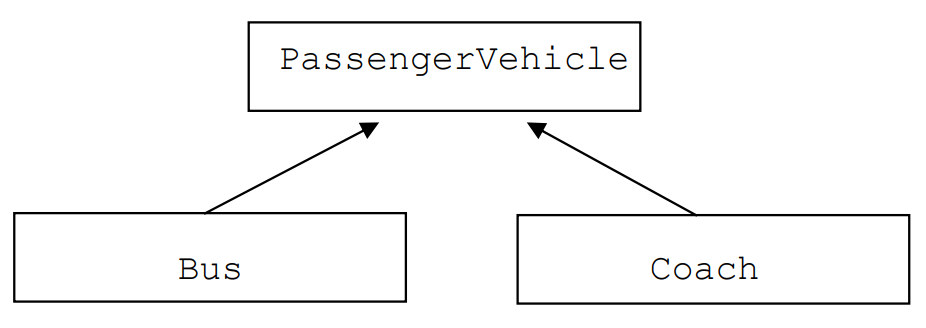
\includegraphics[width=0.35\paperwidth]{C:/Users/Admin/Desktop/Github/question_bank/LyX/static/img/9597-HCI-2016-P1-Q3-1}
\par\end{center}

\subsection*{Task 3.3 }

Write program code for the three classes shown. Evidence 12: Program
code for the three classes. \hfill{}{[}6{]}

\subsection*{Task 3.4 }

The data in \texttt{VEHICLE.dat} does not currently contain the following
additional data: 
\begin{itemize}
\item MaxStanding 
\item SeatBeltsFitted 
\end{itemize}
Write code to read a record from \texttt{VEHICLE.dat} and write the
updated record to \texttt{UVEHICLE.dat}.

As the data on each vehicle is read it should be displayed and the
user should be allowed to input the additional data required.

The user should be prompted to input the data item appropriate to
the type of vehicle.

The number of standing passengers is never more than 15.

For a \textquoteleft \texttt{C}\textquoteright{} type vehicle the
\texttt{MaxStanding} field should contain a zero value. 

The \texttt{SeatBeltsFitted} field should contain an appropriate value.
You are expected to make use of the classes you designed in Task 3.3.

\subsection*{Evidence 13: }

Program code for Task 3.4.\hfill{} {[}10{]}

\subsection*{Evidence 14: }

Screenshot showing the contents of \texttt{UVEHICLE.dat} from running
the program.\hfill{} {[}2{]}